\documentclass{beamer}
\usepackage[utf8]{inputenc}
\usepackage[portuguese]{babel}
\usepackage[demo]{graphicx}
%\usepackage{graphicx}
%\usepackage{subfig}
%\usepackage{subcaption}
%\graphicspath{{images/}}

%% Definindo o Autor e o título
\author{Gustavo Juliano Borges \linebreak Victor Emanuel Almeida \linebreak Marco Guerra Pedroso}
\title{Apresentação~-~Projeto Introdução Engenharia de Software}
\date{Outubro~-~2020}

\usetheme{Ilmenau}
\usetheme{Copenhagen}
\usecolortheme{default}

\begin{document}

	\frame{\titlepage}

	\begin{frame}
		\frametitle{Tópicos}
		\tableofcontents
	\end{frame}

	\section{Introdução}
	\begin{frame}
		\frametitle{Aspectos gerais}
		%\textbf{\Large Informações do Software}
		\begin{itemize}
			\item Data Streaming Video System \textit{(DSVS)} \linebreak
			
			\item Implementado em linguagem C++ \linebreak
			
			\item Aproximadamente 7000 linhas de código \linebreak
		\end{itemize}
	\end{frame}

	\section{Diagrama UML}
	\begin{frame}
		\frametitle{Diagrama}
		\begin{figure}[!htb]
			\centering
			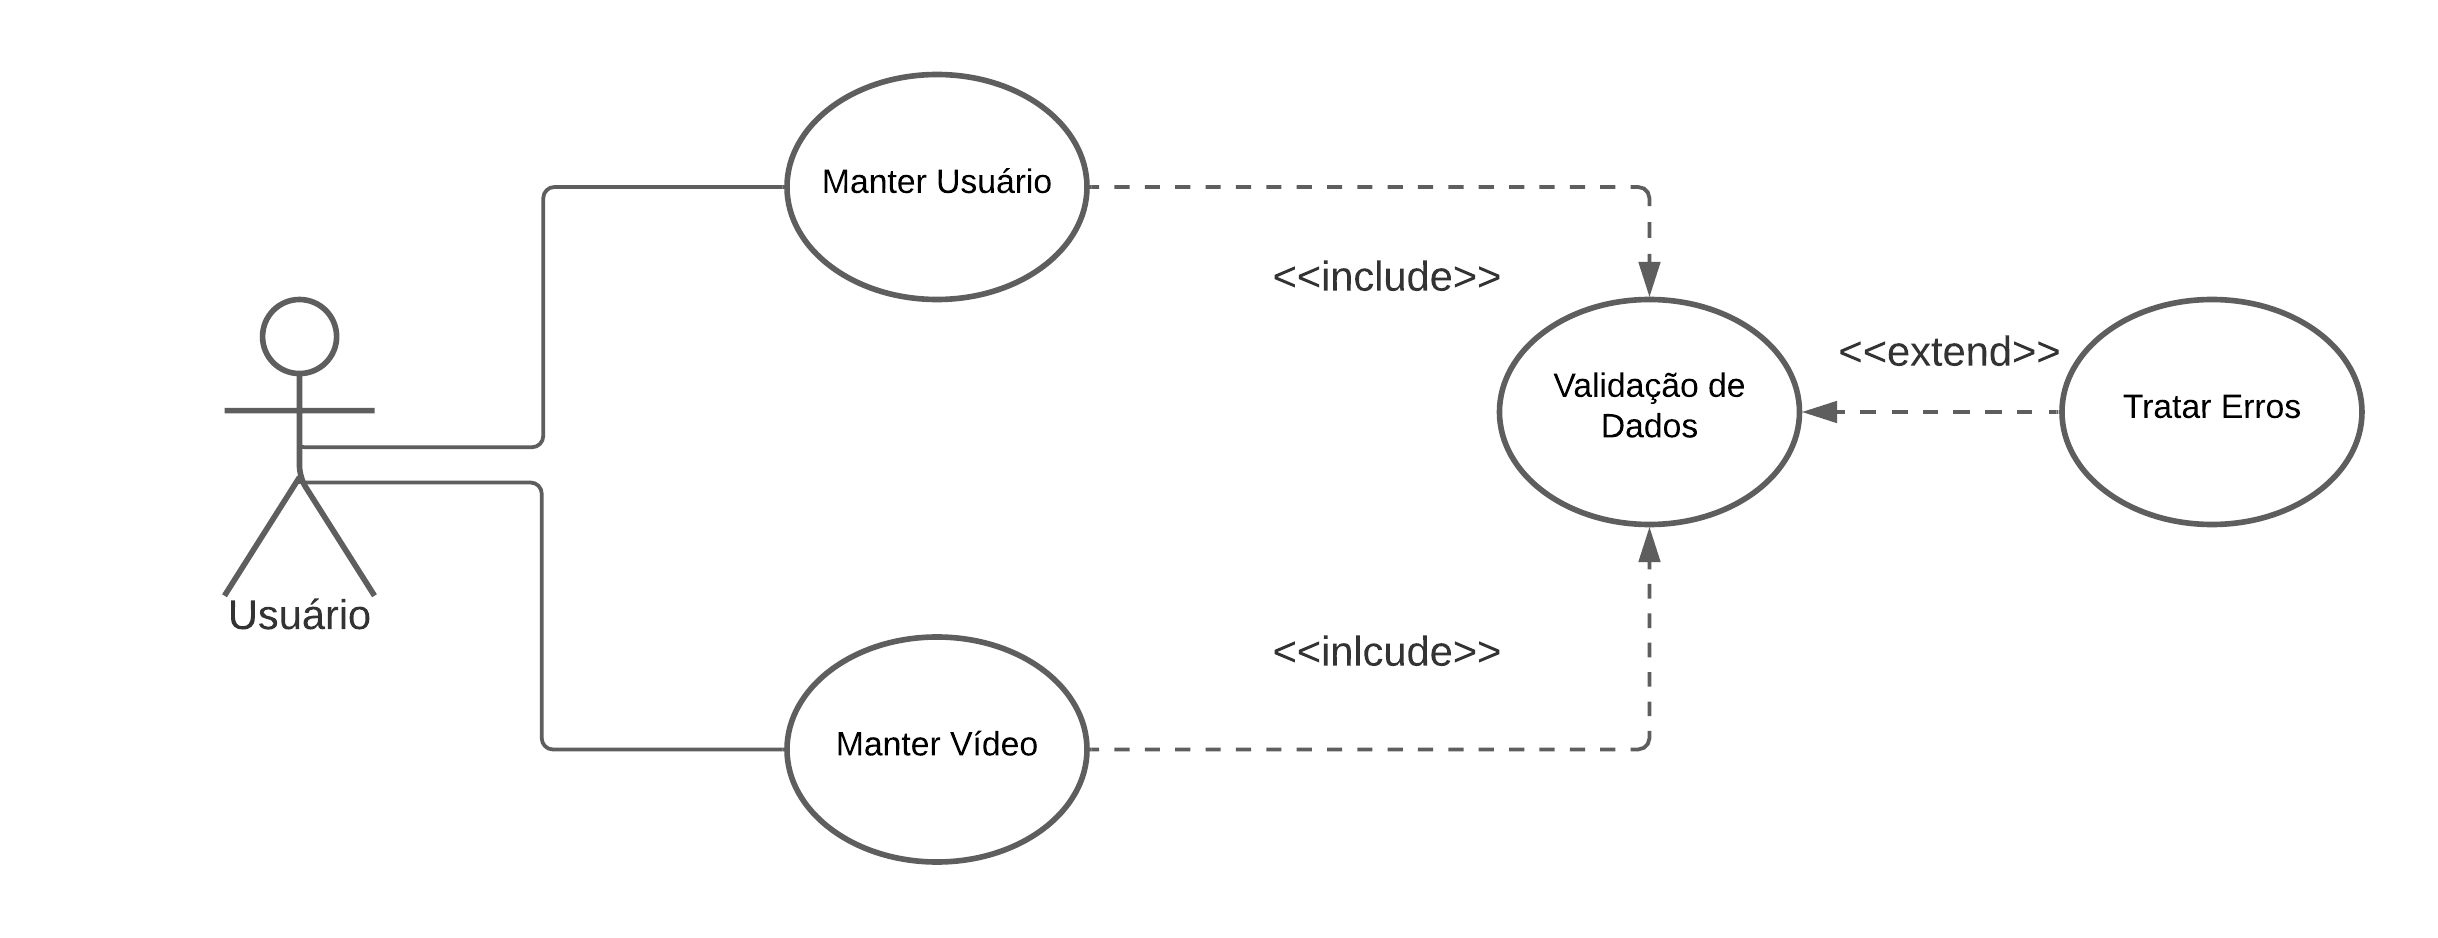
\includegraphics[scale=.5]{images/DiagramaUML.png}
			\caption{\label{fig:}Diagrama UML de casos de uso de um sistema de streaming}
		\end{figure}
	\end{frame}

	\section{Implementação}
	\begin{frame}
		\frametitle{Conteúdo do main}
		O nosso arquivo main é dividido em:
		\begin{enumerate}
			\item leitura do arquivo;
			\item menu principal;
			\item escrita no arquivo;
		\end{enumerate}
	\end{frame}

	\begin{frame}
		\frametitle{Leitura do arquivo}
		\begin{figure}[!htb]
			\begin{subfigure}
				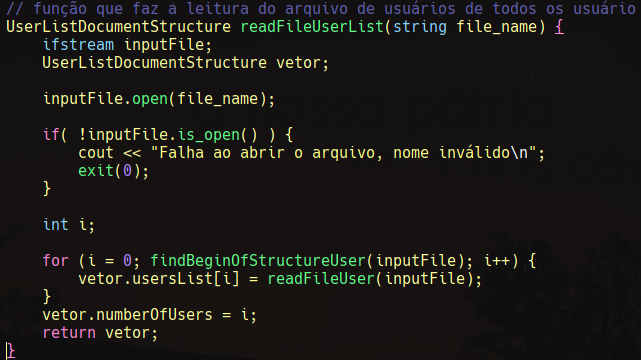
\includegraphics[keepaspectratio, width=.45\textwidth]{images/leArquivoUser.png}
			\end{subfigure}
			\begin{subfigure}
				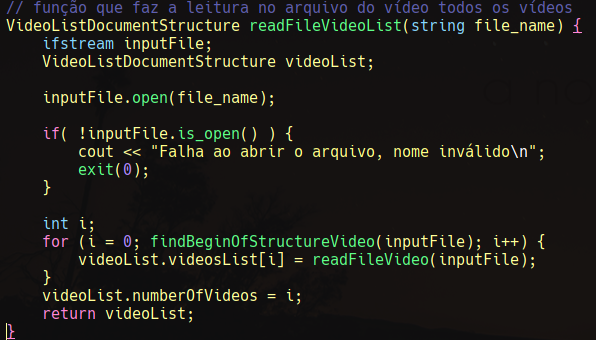
\includegraphics[keepaspectratio, width=.45\textwidth]{images/leArquivoVideo.png}
			\end{subfigure}
			\caption{\label{fig:leitura}Leitura dos vetores do arquivo}
		\end{figure}
	\end{frame}

	\begin{frame}
		\frametitle{Menu principal}
		\begin{figure}[!htb]
			\centering
			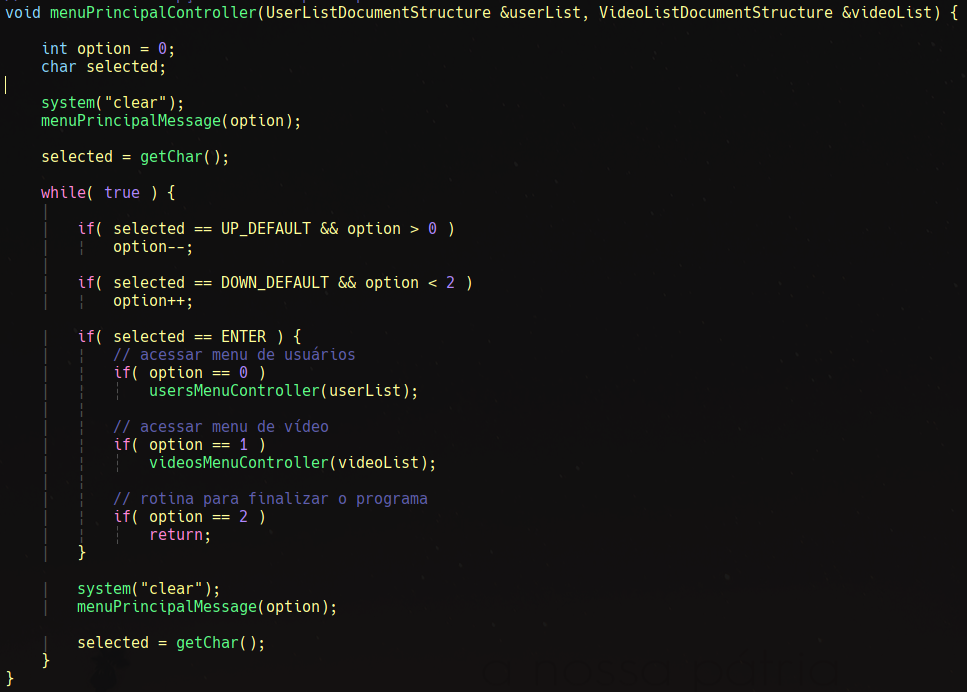
\includegraphics[keepaspectratio, width=.60\textwidth]{images/MenuPrincipal.png}
			\caption{\label{fig:leitura} Interface do Menu principal}
		\end{figure}
	\end{frame}

	\begin{frame}
		\frametitle{Escrita no arquivo}
		\begin{figure}[!htb]
			\centering
			\begin{subfigure}
				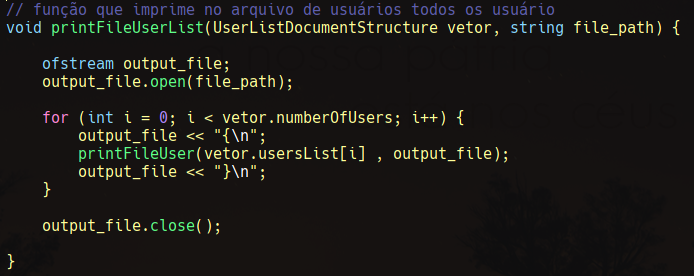
\includegraphics[keepaspectratio, width=.45\textwidth]{images/escreveArquivoUser.png}
			\end{subfigure}
			\begin{subfigure}
				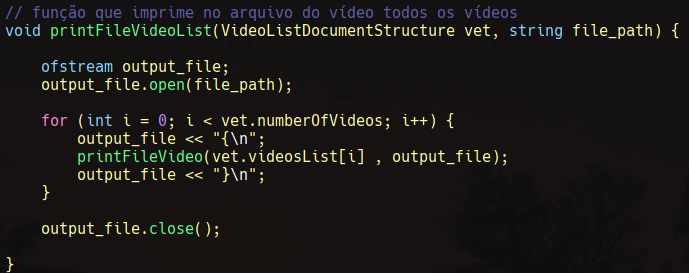
\includegraphics[keepaspectratio, width=.45\textwidth]{images/escreveArquivoVideo.png}
			\end{subfigure}
			\caption{\label{fig:leitura}Escrita dos vetores do arquivo}
		\end{figure}
	\end{frame}
	
	\section{Encerramento}
	\begin{frame}
		\frametitle{Perguntas?}
		\begin{figure}[!htb]
			Obrigado!
		\end{figure}
	\end{frame}

\end{document}
